% Created by tikzDevice version 0.12.6 on 2025-04-02 11:32:06
% !TEX encoding = UTF-8 Unicode
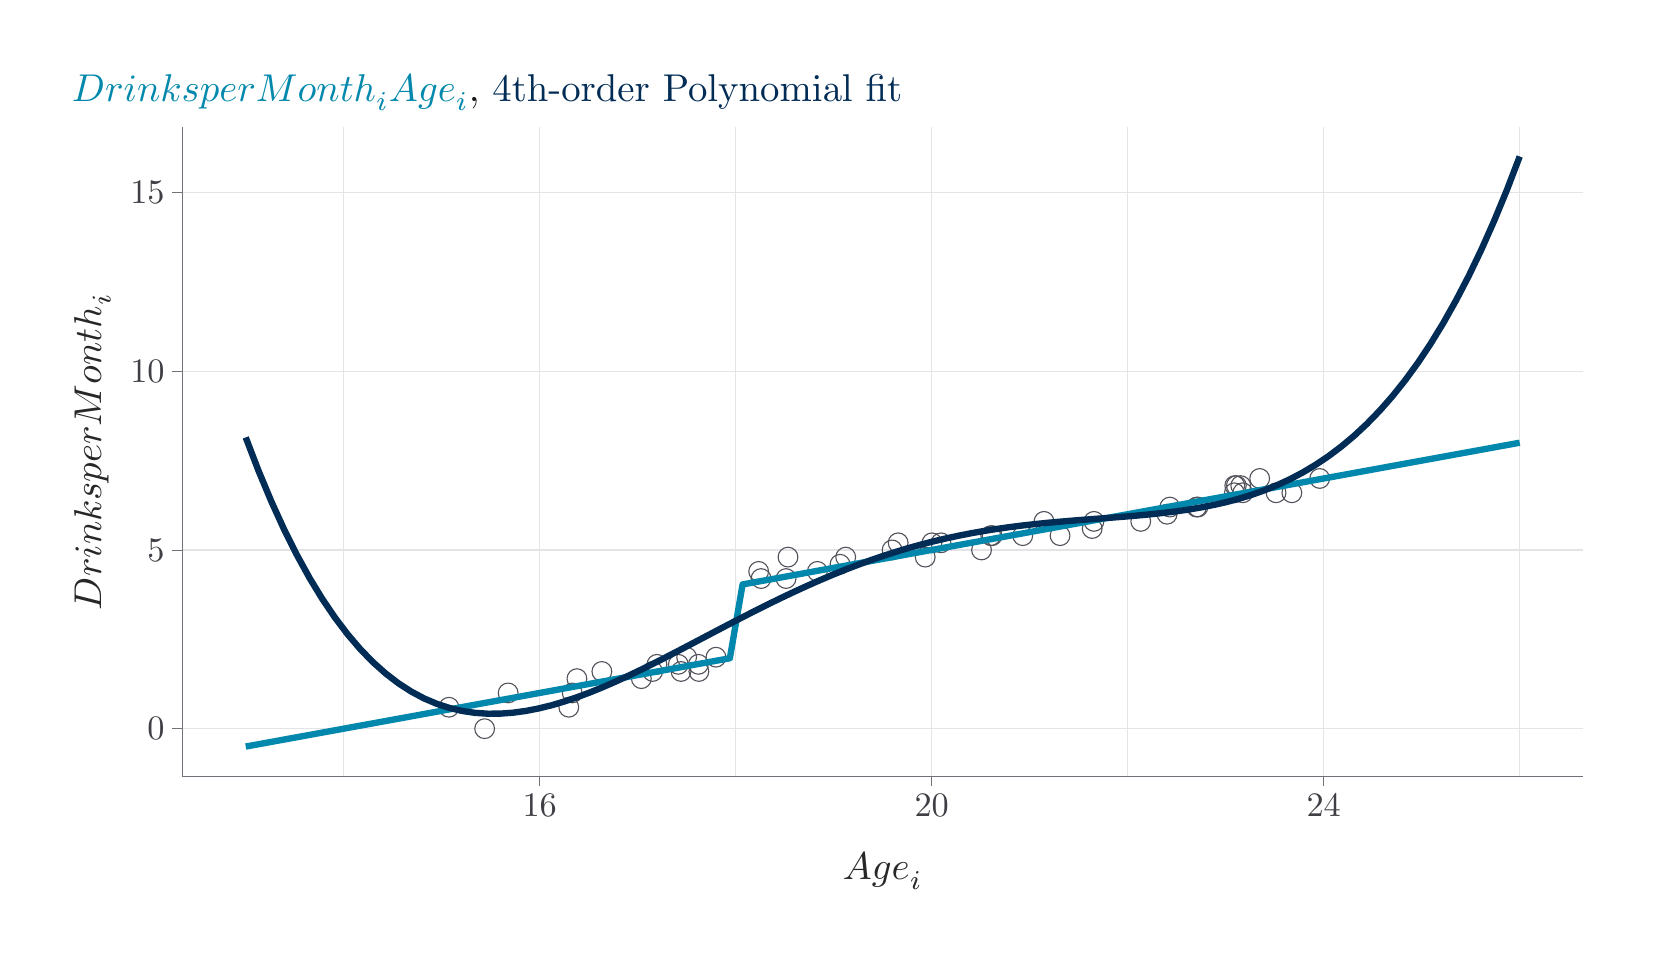
\begin{tikzpicture}[x=1pt,y=1pt]
\definecolor{fillColor}{RGB}{255,255,255}
\path[use as bounding box,fill=fillColor] (0,0) rectangle (578.16,325.21);
\begin{scope}
\path[clip] (  0.00,  0.00) rectangle (578.16,325.21);
\definecolor{drawColor}{RGB}{255,255,255}

\path[draw=drawColor,line width= 0.7pt,line join=round,line cap=round,fill=fillColor] (  0.00,  0.00) rectangle (578.16,325.21);
\end{scope}
\begin{scope}
\path[clip] ( 55.77, 54.78) rectangle (562.16,289.31);
\definecolor{drawColor}{RGB}{255,255,255}
\definecolor{fillColor}{RGB}{255,255,255}

\path[draw=drawColor,line width= 0.7pt,line join=round,line cap=round,fill=fillColor] ( 55.77, 54.78) rectangle (562.16,289.31);
\definecolor{drawColor}{RGB}{228,228,231}

\path[draw=drawColor,line width= 0.4pt,line join=round] (114.20, 54.78) --
	(114.20,289.31);

\path[draw=drawColor,line width= 0.4pt,line join=round] (255.85, 54.78) --
	(255.85,289.31);

\path[draw=drawColor,line width= 0.4pt,line join=round] (397.50, 54.78) --
	(397.50,289.31);

\path[draw=drawColor,line width= 0.4pt,line join=round] (539.14, 54.78) --
	(539.14,289.31);

\path[draw=drawColor,line width= 0.4pt,line join=round] ( 55.77, 71.90) --
	(562.16, 71.90);

\path[draw=drawColor,line width= 0.4pt,line join=round] ( 55.77,136.48) --
	(562.16,136.48);

\path[draw=drawColor,line width= 0.4pt,line join=round] ( 55.77,201.06) --
	(562.16,201.06);

\path[draw=drawColor,line width= 0.4pt,line join=round] ( 55.77,265.63) --
	(562.16,265.63);

\path[draw=drawColor,line width= 0.4pt,line join=round] (185.03, 54.78) --
	(185.03,289.31);

\path[draw=drawColor,line width= 0.4pt,line join=round] (326.67, 54.78) --
	(326.67,289.31);

\path[draw=drawColor,line width= 0.4pt,line join=round] (468.32, 54.78) --
	(468.32,289.31);
\definecolor{drawColor}{RGB}{82,82,91}

\path[draw=drawColor,line width= 0.4pt,line join=round,line cap=round] (242.37, 95.15) circle (  3.57);

\path[draw=drawColor,line width= 0.4pt,line join=round,line cap=round] (236.09, 92.57) circle (  3.57);

\path[draw=drawColor,line width= 0.4pt,line join=round,line cap=round] (173.62, 84.82) circle (  3.57);

\path[draw=drawColor,line width= 0.4pt,line join=round,line cap=round] (225.82, 92.57) circle (  3.57);

\path[draw=drawColor,line width= 0.4pt,line join=round,line cap=round] (165.12, 71.90) circle (  3.57);

\path[draw=drawColor,line width= 0.4pt,line join=round,line cap=round] (326.76,139.06) circle (  3.57);

\path[draw=drawColor,line width= 0.4pt,line join=round,line cap=round] (242.54, 92.57) circle (  3.57);

\path[draw=drawColor,line width= 0.4pt,line join=round,line cap=round] (265.01,126.15) circle (  3.57);

\path[draw=drawColor,line width= 0.4pt,line join=round,line cap=round] (348.00,141.65) circle (  3.57);

\path[draw=drawColor,line width= 0.4pt,line join=round,line cap=round] (295.60,133.90) circle (  3.57);

\path[draw=drawColor,line width= 0.4pt,line join=round,line cap=round] (436.75,159.73) circle (  3.57);

\path[draw=drawColor,line width= 0.4pt,line join=round,line cap=round] (412.70,151.98) circle (  3.57);

\path[draw=drawColor,line width= 0.4pt,line join=round,line cap=round] (264.14,128.73) circle (  3.57);

\path[draw=drawColor,line width= 0.4pt,line join=round,line cap=round] (402.20,146.81) circle (  3.57);

\path[draw=drawColor,line width= 0.4pt,line join=round,line cap=round] (195.53, 79.65) circle (  3.57);

\path[draw=drawColor,line width= 0.4pt,line join=round,line cap=round] (248.71, 97.73) circle (  3.57);

\path[draw=drawColor,line width= 0.4pt,line join=round,line cap=round] (238.12, 97.73) circle (  3.57);

\path[draw=drawColor,line width= 0.4pt,line join=round,line cap=round] (196.77, 84.82) circle (  3.57);

\path[draw=drawColor,line width= 0.4pt,line join=round,line cap=round] (274.04,126.15) circle (  3.57);

\path[draw=drawColor,line width= 0.4pt,line join=round,line cap=round] (436.18,159.73) circle (  3.57);

\path[draw=drawColor,line width= 0.4pt,line join=round,line cap=round] (384.65,144.23) circle (  3.57);

\path[draw=drawColor,line width= 0.4pt,line join=round,line cap=round] (293.54,131.31) circle (  3.57);

\path[draw=drawColor,line width= 0.4pt,line join=round,line cap=round] (274.74,133.90) circle (  3.57);

\path[draw=drawColor,line width= 0.4pt,line join=round,line cap=round] (411.72,149.39) circle (  3.57);

\path[draw=drawColor,line width= 0.4pt,line join=round,line cap=round] (439.06,157.14) circle (  3.57);

\path[draw=drawColor,line width= 0.4pt,line join=round,line cap=round] (312.36,136.48) circle (  3.57);

\path[draw=drawColor,line width= 0.4pt,line join=round,line cap=round] (207.48, 92.57) circle (  3.57);

\path[draw=drawColor,line width= 0.4pt,line join=round,line cap=round] (436.04,157.14) circle (  3.57);

\path[draw=drawColor,line width= 0.4pt,line join=round,line cap=round] (285.36,128.73) circle (  3.57);

\path[draw=drawColor,line width= 0.4pt,line join=round,line cap=round] (438.35,159.73) circle (  3.57);

\path[draw=drawColor,line width= 0.4pt,line join=round,line cap=round] (466.88,162.31) circle (  3.57);

\path[draw=drawColor,line width= 0.4pt,line join=round,line cap=round] (451.10,157.14) circle (  3.57);

\path[draw=drawColor,line width= 0.4pt,line join=round,line cap=round] (348.49,141.65) circle (  3.57);

\path[draw=drawColor,line width= 0.4pt,line join=round,line cap=round] (385.30,146.81) circle (  3.57);

\path[draw=drawColor,line width= 0.4pt,line join=round,line cap=round] (422.37,151.98) circle (  3.57);

\path[draw=drawColor,line width= 0.4pt,line join=round,line cap=round] (359.57,141.65) circle (  3.57);

\path[draw=drawColor,line width= 0.4pt,line join=round,line cap=round] (235.12, 95.15) circle (  3.57);

\path[draw=drawColor,line width= 0.4pt,line join=round,line cap=round] (330.03,139.06) circle (  3.57);

\path[draw=drawColor,line width= 0.4pt,line join=round,line cap=round] (456.81,157.14) circle (  3.57);

\path[draw=drawColor,line width= 0.4pt,line join=round,line cap=round] (314.55,139.06) circle (  3.57);

\path[draw=drawColor,line width= 0.4pt,line join=round,line cap=round] (227.39, 95.15) circle (  3.57);

\path[draw=drawColor,line width= 0.4pt,line join=round,line cap=round] (445.18,162.31) circle (  3.57);

\path[draw=drawColor,line width= 0.4pt,line join=round,line cap=round] (344.67,136.48) circle (  3.57);

\path[draw=drawColor,line width= 0.4pt,line join=round,line cap=round] (422.87,151.98) circle (  3.57);

\path[draw=drawColor,line width= 0.4pt,line join=round,line cap=round] (221.75, 89.98) circle (  3.57);

\path[draw=drawColor,line width= 0.4pt,line join=round,line cap=round] (198.47, 89.98) circle (  3.57);

\path[draw=drawColor,line width= 0.4pt,line join=round,line cap=round] (367.25,146.81) circle (  3.57);

\path[draw=drawColor,line width= 0.4pt,line join=round,line cap=round] (373.05,141.65) circle (  3.57);

\path[draw=drawColor,line width= 0.4pt,line join=round,line cap=round] (152.22, 79.65) circle (  3.57);

\path[draw=drawColor,line width= 0.4pt,line join=round,line cap=round] (324.32,133.90) circle (  3.57);
\definecolor{drawColor}{RGB}{1,136,172}

\path[draw=drawColor,line width= 2.3pt,line join=round] ( 78.79, 65.44) --
	( 83.40, 66.28) --
	( 88.00, 67.12) --
	( 92.60, 67.96) --
	( 97.21, 68.80) --
	(101.81, 69.64) --
	(106.41, 70.48) --
	(111.02, 71.32) --
	(115.62, 72.16) --
	(120.22, 73.00) --
	(124.83, 73.84) --
	(129.43, 74.68) --
	(134.03, 75.52) --
	(138.64, 76.36) --
	(143.24, 77.20) --
	(147.84, 78.04) --
	(152.45, 78.88) --
	(157.05, 79.72) --
	(161.66, 80.56) --
	(166.26, 81.40) --
	(170.86, 82.23) --
	(175.47, 83.07) --
	(180.07, 83.91) --
	(184.67, 84.75) --
	(189.28, 85.59) --
	(193.88, 86.43) --
	(198.48, 87.27) --
	(203.09, 88.11) --
	(207.69, 88.95) --
	(212.29, 89.79) --
	(216.90, 90.63) --
	(221.50, 91.47) --
	(226.10, 92.31) --
	(230.71, 93.15) --
	(235.31, 93.99) --
	(239.91, 94.83) --
	(244.52, 95.67) --
	(249.12, 96.51) --
	(253.73, 97.35) --
	(258.33,124.02) --
	(262.93,124.86) --
	(267.54,125.69) --
	(272.14,126.53) --
	(276.74,127.37) --
	(281.35,128.21) --
	(285.95,129.05) --
	(290.55,129.89) --
	(295.16,130.73) --
	(299.76,131.57) --
	(304.36,132.41) --
	(308.97,133.25) --
	(313.57,134.09) --
	(318.17,134.93) --
	(322.78,135.77) --
	(327.38,136.61) --
	(331.98,137.45) --
	(336.59,138.29) --
	(341.19,139.13) --
	(345.80,139.97) --
	(350.40,140.81) --
	(355.00,141.65) --
	(359.61,142.48) --
	(364.21,143.32) --
	(368.81,144.16) --
	(373.42,145.00) --
	(378.02,145.84) --
	(382.62,146.68) --
	(387.23,147.52) --
	(391.83,148.36) --
	(396.43,149.20) --
	(401.04,150.04) --
	(405.64,150.88) --
	(410.24,151.72) --
	(414.85,152.56) --
	(419.45,153.40) --
	(424.05,154.24) --
	(428.66,155.08) --
	(433.26,155.92) --
	(437.87,156.76) --
	(442.47,157.60) --
	(447.07,158.44) --
	(451.68,159.27) --
	(456.28,160.11) --
	(460.88,160.95) --
	(465.49,161.79) --
	(470.09,162.63) --
	(474.69,163.47) --
	(479.30,164.31) --
	(483.90,165.15) --
	(488.50,165.99) --
	(493.11,166.83) --
	(497.71,167.67) --
	(502.31,168.51) --
	(506.92,169.35) --
	(511.52,170.19) --
	(516.12,171.03) --
	(520.73,171.87) --
	(525.33,172.71) --
	(529.94,173.55) --
	(534.54,174.39) --
	(539.14,175.23);
\definecolor{drawColor}{RGB}{0,44,85}

\path[draw=drawColor,line width= 2.3pt,line join=round] ( 78.79,177.14) --
	( 83.40,165.14) --
	( 88.00,154.12) --
	( 92.60,144.02) --
	( 97.21,134.81) --
	(101.81,126.43) --
	(106.41,118.87) --
	(111.02,112.07) --
	(115.62,105.99) --
	(120.22,100.61) --
	(124.83, 95.88) --
	(129.43, 91.78) --
	(134.03, 88.26) --
	(138.64, 85.29) --
	(143.24, 82.84) --
	(147.84, 80.88) --
	(152.45, 79.38) --
	(157.05, 78.30) --
	(161.66, 77.62) --
	(166.26, 77.31) --
	(170.86, 77.34) --
	(175.47, 77.69) --
	(180.07, 78.32) --
	(184.67, 79.22) --
	(189.28, 80.35) --
	(193.88, 81.71) --
	(198.48, 83.25) --
	(203.09, 84.97) --
	(207.69, 86.84) --
	(212.29, 88.84) --
	(216.90, 90.95) --
	(221.50, 93.15) --
	(226.10, 95.43) --
	(230.71, 97.76) --
	(235.31,100.14) --
	(239.91,102.55) --
	(244.52,104.97) --
	(249.12,107.39) --
	(253.73,109.80) --
	(258.33,112.18) --
	(262.93,114.53) --
	(267.54,116.83) --
	(272.14,119.08) --
	(276.74,121.26) --
	(281.35,123.38) --
	(285.95,125.41) --
	(290.55,127.37) --
	(295.16,129.24) --
	(299.76,131.01) --
	(304.36,132.69) --
	(308.97,134.27) --
	(313.57,135.75) --
	(318.17,137.14) --
	(322.78,138.42) --
	(327.38,139.60) --
	(331.98,140.68) --
	(336.59,141.67) --
	(341.19,142.57) --
	(345.80,143.38) --
	(350.40,144.11) --
	(355.00,144.76) --
	(359.61,145.34) --
	(364.21,145.85) --
	(368.81,146.32) --
	(373.42,146.73) --
	(378.02,147.12) --
	(382.62,147.48) --
	(387.23,147.83) --
	(391.83,148.17) --
	(396.43,148.53) --
	(401.04,148.92) --
	(405.64,149.36) --
	(410.24,149.85) --
	(414.85,150.42) --
	(419.45,151.08) --
	(424.05,151.85) --
	(428.66,152.76) --
	(433.26,153.81) --
	(437.87,155.04) --
	(442.47,156.46) --
	(447.07,158.10) --
	(451.68,159.98) --
	(456.28,162.12) --
	(460.88,164.56) --
	(465.49,167.31) --
	(470.09,170.40) --
	(474.69,173.86) --
	(479.30,177.72) --
	(483.90,182.01) --
	(488.50,186.75) --
	(493.11,191.99) --
	(497.71,197.74) --
	(502.31,204.05) --
	(506.92,210.95) --
	(511.52,218.46) --
	(516.12,226.64) --
	(520.73,235.50) --
	(525.33,245.10) --
	(529.94,255.47) --
	(534.54,266.63) --
	(539.14,278.65);
\end{scope}
\begin{scope}
\path[clip] (  0.00,  0.00) rectangle (578.16,325.21);
\definecolor{drawColor}{RGB}{113,113,122}

\path[draw=drawColor,line width= 0.3pt,line join=round] ( 55.77, 54.78) --
	( 55.77,289.31);
\end{scope}
\begin{scope}
\path[clip] (  0.00,  0.00) rectangle (578.16,325.21);
\definecolor{drawColor}{RGB}{63,63,70}

\node[text=drawColor,anchor=base east,inner sep=0pt, outer sep=0pt, scale=  1.24] at ( 49.47, 67.82) {0};

\node[text=drawColor,anchor=base east,inner sep=0pt, outer sep=0pt, scale=  1.24] at ( 49.47,132.40) {5};

\node[text=drawColor,anchor=base east,inner sep=0pt, outer sep=0pt, scale=  1.24] at ( 49.47,196.98) {10};

\node[text=drawColor,anchor=base east,inner sep=0pt, outer sep=0pt, scale=  1.24] at ( 49.47,261.55) {15};
\end{scope}
\begin{scope}
\path[clip] (  0.00,  0.00) rectangle (578.16,325.21);
\definecolor{drawColor}{RGB}{113,113,122}

\path[draw=drawColor,line width= 0.3pt,line join=round] ( 52.27, 71.90) --
	( 55.77, 71.90);

\path[draw=drawColor,line width= 0.3pt,line join=round] ( 52.27,136.48) --
	( 55.77,136.48);

\path[draw=drawColor,line width= 0.3pt,line join=round] ( 52.27,201.06) --
	( 55.77,201.06);

\path[draw=drawColor,line width= 0.3pt,line join=round] ( 52.27,265.63) --
	( 55.77,265.63);
\end{scope}
\begin{scope}
\path[clip] (  0.00,  0.00) rectangle (578.16,325.21);
\definecolor{drawColor}{RGB}{113,113,122}

\path[draw=drawColor,line width= 0.3pt,line join=round] ( 55.77, 54.78) --
	(562.16, 54.78);
\end{scope}
\begin{scope}
\path[clip] (  0.00,  0.00) rectangle (578.16,325.21);
\definecolor{drawColor}{RGB}{113,113,122}

\path[draw=drawColor,line width= 0.3pt,line join=round] (185.03, 51.28) --
	(185.03, 54.78);

\path[draw=drawColor,line width= 0.3pt,line join=round] (326.67, 51.28) --
	(326.67, 54.78);

\path[draw=drawColor,line width= 0.3pt,line join=round] (468.32, 51.28) --
	(468.32, 54.78);
\end{scope}
\begin{scope}
\path[clip] (  0.00,  0.00) rectangle (578.16,325.21);
\definecolor{drawColor}{RGB}{63,63,70}

\node[text=drawColor,anchor=base,inner sep=0pt, outer sep=0pt, scale=  1.24] at (185.03, 40.32) {16};

\node[text=drawColor,anchor=base,inner sep=0pt, outer sep=0pt, scale=  1.24] at (326.67, 40.32) {20};

\node[text=drawColor,anchor=base,inner sep=0pt, outer sep=0pt, scale=  1.24] at (468.32, 40.32) {24};
\end{scope}
\begin{scope}
\path[clip] (  0.00,  0.00) rectangle (578.16,325.21);
\definecolor{drawColor}{RGB}{39,39,42}

\node[text=drawColor,anchor=base,inner sep=0pt, outer sep=0pt, scale=  1.40] at (308.97, 17.36) {$\text{Age}_i$};
\end{scope}
\begin{scope}
\path[clip] (  0.00,  0.00) rectangle (578.16,325.21);
\definecolor{drawColor}{RGB}{39,39,42}

\node[text=drawColor,rotate= 90.00,anchor=base,inner sep=0pt, outer sep=0pt, scale=  1.40] at ( 26.54,172.05) {$\text{Drinks per Month}_i$};
\end{scope}
\begin{scope}
\path[clip] (  0.00,  0.00) rectangle (578.16,325.21);
\definecolor{drawColor}{RGB}{24,24,27}

\node[text=drawColor,anchor=base west,inner sep=0pt, outer sep=0pt, scale=  1.40] at ( 16.00,298.67) {{\color[HTML]{0188AC} $\expec{\text{Drinks per Month}_i}{\text{Age}_i}$}, {\color[HTML]{002C55} 4th-order Polynomial fit}};
\end{scope}
\end{tikzpicture}
